\chapter{Introduction}\label{ch-introduction}
\thispagestyle{headings}
\markboth{Chapter \ref{ch-introduction}: Introduction}{Chapter \ref{ch-introduction}: Introduction}

QUESO is a parallel object-oriented statistical library dedicated to the research of statistically robust, scalable, load balanced, and fault-tolerant mathematical algorithms for the quantification of uncertainty (UQ) of mathematical models and their predictions. 
% It has been developed to implement advanced algorithms for Bayesian
% inference, including are many variants of MCMC and the multi-level algorithm.  It is able to handle uni- and multi-processor Linux
% environments and to provide a wide range of diagnostics.


The purpose of this chapter is to introduce relevant terminology, mathematical and statistical concepts, statistical algorithms, together with an overall description of how the user's application may be linked with the QUESO library.



\section{Preliminaries}


Statistical inverse theory reformulates inverse problems as problems of statistical inference by means of Bayesian statistics: all quantities are modeled as random variables, and probability distribution of the quantities encapsulates the uncertainty observed in their values. The solution to the inverse problem is then the probability distribution of the quantity of interest when all information available has been incorporated in the model. This (posterior) distribution describes the degree of confidence about the quantity after the measurement has been performed \cite{KaSo05}.

Thus, the solution to the statistical inverse problem may be given by Bayes' formula, which express the posterior distribution as a function of the prior distribution and the data represented through the likelihood function.

The likelihood function has an open form and its evaluation is highly computationally expensive.  Moreover, simulation-based posterior inference requires a large number of forward calculations to be performed, therefore fast and efficient sampling techniques are required for posterior inference.

It is often not straightforward to obtain explicit posterior point estimates of the solution, since it usually involves the evaluation of a high-dimensional integral with respect to a possibly non-smooth posterior distribution. In such cases, an alternative integration technique is the Markov chain Monte Carlo method: posterior means may be estimated using the sample mean from a series of random draws from the posterior distribution.

QUESO is designed in an abstract way so that it can be used by any computational model, as long as a likelihood function (in the case of statistical inverse problems) and a quantity of interest (QoI) function (in the case of statistical forward problems) is provided by the user application.

QUESO provides tools for both sampling algorithms for statistical inverse problems, following Bayes' formula, and statistical forward problems. It contains Monte Carlo solvers (for autocorrelation, kernel density estimation and accuracy assessment), MCMC (e.g. Metropolis Hastings \cite{Metr_1953,Hast_1970}) as well as the DRAM \cite{HaLaMiSa06} (for sampling from probability distributions); it also has the capacity to handle many chains or sequences in parallel, each chain or sequence itself demanding many computing nodes because of the computational model being statistically explored \cite{PrSc12}.

\section{Key Statistical Concepts}\label{sec:statistical_concepts}

A computational model is a combination of a
mathematical model and a discretization that enables the approximate
solution of the mathematical model using computer algorithms and  might be used in two different types of problems:
forward or inverse. 

Any computational model is composed of a vector $\boldsymbol{\theta}$ of $n$ {\it parameters}, {\it state variables} $\mathbf{u}$, and {\it state equations} $\mathbf{r}(\boldsymbol{\theta},\mathbf{u}) = \mathbf{0}$.
Once the solution $\mathbf{u}$ is available, the computational model also includes extra functions for e.g.
the calculation of {\it model output data} $\mathbf{y} = \mathbf{y}(\boldsymbol{\theta},\mathbf{u})$, and the {\it prediction} of a
vector $\mathbf{q} = \mathbf{q}(\boldsymbol{\theta},\mathbf{u})$ of $m$~quantities~of~interest\text{ (QoI)},

Parameters designate all model variables that are neither state variables
nor further quantities computed by the model, such as: material properties, coefficients, constitutive parameters, boundary conditions, initial conditions,
external forces, parameters for modeling the model error, characteristics of an experimental apparatus (collection of devices and procedures),
discretization choices and numerical algorithm options.

% Some parameters might be directly measurable, e.g. room temperature,
% but some may not, e.g. a material property.
% Parameters that cannot be measured directly need to be {\it estimated}
% through the solution of an {\it inverse problem}.


In the case of a forward problem, the parameters $\boldsymbol{\theta}$ are given and
one then needs to compute $\mathbf{u}$, $\mathbf{y}$ and/or $\mathbf{q}$.
In the case of an inverse problem, however, experimental data $\mathbf{d}$ is given and
one then needs to {\it estimate} the values of the parameters $\boldsymbol{\theta}$ that
cause $\mathbf{y}$ to best fit  $\mathbf{d}$.
%where ``best'' is an algorithm dependent concept.

%The process of parameter estimation is also referred to as model calibration or model update, and it usually precedes the computation of a QoI, a process called model prediction. 

Figure~\ref{fig-generic-problems} represents general inverse and forward problems respectively.
%
\begin{figure*}[htb]
\begin{minipage}[b]{0.5\textwidth}
\input{rawfigs/gfp01.latex}\\
\centering
(a)
\end{minipage}%\hfill
\begin{minipage}[b]{0.5\textwidth}
\input{rawfigs/gip01.latex}\\
\centering 
(b)
\end{minipage}
%\end{center}
\vspace{-20pt}
\caption{The representation of (a) a generic forward problem and (b) a generic inverse problem.}
\label{fig-generic-problems}
\end{figure*}


There are many possible sources of uncertainty on a computational model. %procedures (a) and (b) above. 
First, $\mathbf{d}$ need not be equal to the actual values of observables because of errors in the measurement process. Second, the values of the input parameters to the phenomenon might not be precisely known. Third, the appropriate set of
equations governing the phenomenon might not be well understood. 

Computational models can be classified as either deterministic or stochastic -- which are the ones of interest here.  In deterministic models, all parameters are assigned numbers, and no parameter is related to the parametrization of a random variable (RV) or field. As a
consequence, a deterministic model assigns a number to each of the components of quantities $\mathbf{u}$, $\mathbf{y}$ and $\mathbf{q}$. In stochastic models, however, at least one parameter is assigned a probability density function (PDF) or is related to the parametrization of a RV or field, causing $\mathbf{u}$, $\mathbf{y}$ and $\mathbf{q}$ to become random variables.  Note that not all components of $\boldsymbol{\theta}$ need to be treated as random. As long as at least one component is random, $\boldsymbol{\theta}$ is a random vector, and the problem is stochastic.



In the case of forward problems, statistical forward problems can be represented very similarly to deterministic forward problems,
as seen in Figure \ref{fig-sfp-queso}.
In the case of inverse problems, as depicted in Figure \ref{fig-sip-queso}, however, the conceptual connection between deterministic and statistical problems
is not as straightforward.

\begin{figure}[h!]
\centerline{
\input{rawfigs/sfp01.latex}\\
}
\caption{
The representation of a statistical forward problem.
$\boldsymbol{\Theta}$ denotes a random variable related to parameters,
$\boldsymbol{\theta}$ denotes a realization of $\boldsymbol{\Theta}$ and
$\mathbf{Q}$ denotes a random variable related to quantities of interest.
}
\label{fig-sfp-queso}
\end{figure}

\begin{figure}[h!]
\centerline{
\input{rawfigs/sip01.latex}\\
}
\caption{
The representation of a statistical inverse problem.
$\boldsymbol{\Theta}$ denotes a random variable related to parameters,
$\boldsymbol{\theta}$ denotes a realization of $\boldsymbol{\Theta}$ and
$\mathbf{r}$ denotes model equations,
$\mathbf{y}$ denotes some model output data and
$\mathbf{d}$ denotes experimental data.
}
\label{fig-sip-queso}
\end{figure}


QUESO adopts a Bayesian analysis \cite{KaSo05, Ro04} for statistical inverse problems, interpreting the posterior PDF
\begin{equation}\label{eq-Bayes-solution}
\pi_{\text{posterior}}(\boldsymbol{\theta}|\mathbf{d})=\frac{\pi_{\text{prior}}(\boldsymbol{\theta})\pi_{\text{likelihood}}(\mathbf{d}|\boldsymbol{\theta})}{\pi(\mathbf{d})}
\end{equation}
as the solution. Such solutions combine the prior information $\pi_{\text{prior}}(\boldsymbol{\theta})$ of the parameters,
the information $\pi(\mathbf{d})$ on the data, and the likelihood $\pi_{\text{likelihood}}(\mathbf{d}|\boldsymbol{\theta})$ that the model computes certain data values with a given set of input parameters.

This semantic interpretation of achieving a posterior knowledge on the parameters (on the model)
after combining some prior model knowledge with experimental information provides an important mechanism for dealing with uncertainty.
Although mathematically simple, is not computationally trivial. 

% 
% \new{
% 
% 
% 
% \section{Sampling the Posterior Density}
% 
% The generation of a Markov chain of parameter vectors $\mathbf{m}\in\mathbb{R}^N$ demands at least the calculation of values $\mathcal{F}(\mathbf{m})$, where $\mathcal{F}$ is the misfit function.
% A chain generation algorithm might also need the quantities $\nabla\mathcal{F}(\mathbf{m})$ and ${\nabla}^2\mathcal{F}(\mathbf{m})$.
% 
% Target pdf $\pi:\mathbb{R}^N\rightarrow\mathbb{R}$ with support $supp(\pi)$.
% 
% 
% \todo{\subsection{Misfit Functions $\mathcal{F}(\mathbf{m})$}}
% 
% % 
% % 
% % 
% % Let $\mathbf{m}=(A_1,E_1,\ldots,A_{N_{\text{mat}}},,E_{N_{\text{mat}}})$ be the vector of model parameters and $M=\mathbb{R}_{+}^{2N_{\text{mat}}}$ be the space of model parameters.
% % Let
% % $V_T$ denote the space of functions $f:\mathbb{R}_{+}\rightarrow\mathbb{R}_{+}$ that are weakly differentiable.
% % $V_T$ will be the space of temperature profiles.
% % Finally, let
% % $V_w$ denote the space of functions $f:\mathbb{R}_{+}\rightarrow[0,1]$ that are weakly differentiable.
% % $V_w$ will be the space of relative mass evolutions.
% % We will denote by
% % \begin{equation*}
% % w(\mathbf{m},T)\in V_w
% % \end{equation*}
% % the solution of \eqref{eq-composite-sum}-\eqref{eq-composite-initial-values} for given $\mathbf{m}\in M$ and $T\in V_T$.
% % 
% % Let
% % $V_S$ denote the space of all functions $f:\mathbb{R}_{+}\rightarrow\mathbb{R}_{+}$ that are square-Lebesgue-integrable
% % over any finite interval.
% % $V_S$ will be the space of misfit weight functions.
% % Let
% % $V_{\sigma}$ denote the space of all functions $f:\mathbb{R}_{+}\rightarrow\mathbb{R}_+^{*}$ such that $1/f$ is square-Lebesgue-integrable
% % over any finite interval.
% % $V_{\sigma}$ will be the space of variance functions.
% % 
% % Given a reference relative mass evolution function $\text{$d$}\in V_w$,
% % a temperature profile $T\in V_T$,
% % and some $t_{_{\text{F}}}>0$,
% % let $\mathcal{F}:M\rightarrow\mathbb{R}$ be the functional defined by
% % \begin{equation*}
% % \mathcal{F}(\mathbf{m}) = \int_{0}^{t_{_{\text{F}}}}~\left\{[w(\mathbf{m},T)](t)-\text{$d$}(t)\right\}^2\cdot S(t)~dt,
% % \end{equation*}
% % or simply
% % \begin{equation}\label{eq-F}
% % \mathcal{F}(\mathbf{m}) = \int_{0}^{t_{_{\text{F}}}}~(w-d)^2\cdot S~dt.
% % \end{equation}
% % 
% % 
% % The functional \eqref{eq-F} is general enough for our studies, since it can properly describe
% % not only the case where one has continuous measurements $\text{$d$}$,
% % but also the case of a finite set of $N_{\text{meas}}$ discrete measurements $0\leqslant d_j\leqslant 1$,
% % $1\leqslant i\leqslant N_{\text{meas}}$ at instants $0\leqslant t_1 < t_2 < \ldots < t_{N_{\text{meas}}}$.
% % 
% % In the case of continuous measurements, for instance, one can set
% % \begin{equation*}
% % \mathcal{F}_1(\mathbf{m}) = \int_{0}^{t_{_{\text{F}}}}~\left\{[w(\mathbf{m},T)](t)-\text{$d$}(t)\right\}^2\cdot\frac{1}{\sigma^2(t)}~dt,
% % \end{equation*}
% % for some given variance function $\sigma^2\in V_S$ satisfying $\sigma(t)>0$ for all $t\geqslant 0$.
% % 
% % On the other hand, when measurements are discrete and a corresponding finite set of variances $\sigma_j^2>0,~j=1,2,\ldots,N_{\text{meas}}$ is given, one can set
% % \begin{equation*}
% % \mathcal{F}_2(\mathbf{m}) = \int_0^{t_{_F}}~\{[w(\mathbf{m},T)](t)-\hat{d}(t)\}^2\cdot\left[\sum_{j=1}^{N_{\text{meas}}}\frac{\delta(t-t_j)}{{\hat{\sigma}}^2(t)}\right]~dt,
% % \end{equation*}
% % where
% % $\hat{d}\in V_w$ and $\hat{\sigma}\in V_{\sigma}$ are any functions satisfying
% % $\hat{d}(t_j)=d_j$ and $\hat{\sigma}(t_j)=\sigma_j$, $j=1,2,\ldots,N_{\text{meas}}$,
% % in which case the functional simply becomes
% % \begin{equation*}
% % \mathcal{F}_2(\mathbf{m}) = \sum_{j=1}^{N_{\text{meas}}}~\frac{\{[w(\mathbf{m},T)](t_j)-d_j\}^2}{\sigma_j^2},
% % \end{equation*}
% % assuming, without loss of generality, that $t_{_F}\geqslant t_{N_{\text{meas}}}$.
% 
% 
% \subsection{The Metropolis Hastings Algorithm}
% 
% The inputs are:
% \begin{equation}\label{eq-inputs-MH-method}
% \left\{
% \begin{array}{cl}
% 1. & \text{Number }n_{\text{pos}}\geqslant 2\text{ of positions in the chain} \\
% 2. & \text{Initial guess }\mathbf{m}^{(0)} \\
% 3. & \text{Function }q:\mathbb{R}^N\times\mathbb{R}^N\rightarrow\mathbb{R}_{+},\text{ such that }q(\mathbf{a},\cdot)\text{ is a pdf for any }\mathbf{a}\in\mathbb{R}^N
% \end{array}
% \right.
% \end{equation}
% 
% Let us define the function $\alpha:\mathbb{R}^N\times\mathbb{R}^N\rightarrow[0,1]$ defined by
% \begin{equation}\label{eq-alpha}
% \alpha(\mathbf{a},\mathbf{b})=\text{min}\left\{1,\frac{\pi(\mathbf{b})}{\pi(\mathbf{a})}\cdot\frac{q(\mathbf{b},\mathbf{a})}{q(\mathbf{a},\mathbf{b})}\right\}
% \end{equation}
% 
% \begin{equation}\label{eq-MH-method}
% \left\{
% \begin{array}{cl}
% 01. & \text{Do }\{ \\
% 02. & \quad\underline{\text{{\bf Generate candidate}}}~\mathbf{c}\in\mathbb{R}^N\text{ by sampling }q(\mathbf{m}^{(k)},\cdot); \\
% 03. & \quad\text{If }\mathbf{c}\notin supp(\pi)\text{ then set }\mathbf{m}^{(k+1)}=\mathbf{m}^{(k)}; \\
% 04. & \quad\text{If }\mathbf{c}\in supp(\pi)\text{ then }\{ \\
% 05. & \quad\quad\underline{\text{{\bf Compute acceptance probability}}}~\alpha(\mathbf{m}^{(k)},\mathbf{c}); \\
% 06. & \quad\quad\text{Generate a sample }0 < \tau\leqslant 1\text{ from an uniform rv defined over }(0,1]; \\
% 07. & \quad\quad\text{If }\alpha<        \tau\text{ then set }\mathbf{m}^{(k+1)}=\mathbf{m}^{(k)}; \\
% 08. & \quad\quad\text{If }\alpha\geqslant\tau\text{ then set }\mathbf{m}^{(k+1)}=\mathbf{c}; \\
% 09. & \quad\} \\
% 10. & \quad\text{Set }k=k+1; \\
% 11. & \}\text{ while }(k+1 < n_{\text{pos}}).
% \end{array}
% \right.
% \end{equation}
% 
% \subsection{The Metropolis Hastings Algorithm with Delayed Rejection}
% 
% The inputs are:
% \begin{equation}\label{eq-inputs-DR-method}
% \left\{
% \begin{array}{cl}
% 1. & \text{Number }n_{\text{pos}}\geqslant 2\text{ of positions in the chain} \\
% 2. & \text{Initial guess }\mathbf{m}^{(0)} \\
% 3. & n_{\text{stages}}\geqslant 1 \\
% 4. & \text{For }1\leqslant i\leqslant n_{\text{stages}},\text{ functions }q_i:\underbrace{\mathbb{R}^N\times\ldots\times\mathbb{R}^N}_{(i+1)\text{ times}}\rightarrow\mathbb{R}_{+},\text{ such that } \\
%    & q_i(\mathbf{a},\mathbf{x}^{(1)},\ldots,\mathbf{x}^{(i-1)},\cdot)\text{ is a pdf for any }(\mathbf{a},\mathbf{x}^{(1)},\ldots,\mathbf{x}^{(i-1)})\in\underbrace{\mathbb{R}^N\times\ldots\times\mathbb{R}^N}_{i\text{ times}}
% \end{array}
% \right.
% \end{equation}
% 
% We then recursively define
% \begin{equation}\label{eq-alphas}
% \alpha_i:\underbrace{\mathbb{R}^n\times\ldots\times\mathbb{R}^n}_{(i+1)\text{ times}}\rightarrow [0,1],\quad 1\leqslant i\leqslant n_{\text{stages}},
% \end{equation}
% by setting
% \begin{equation*}
% \alpha_1(\mathbf{a},\mathbf{x}^{(1)}) = \text{ min}
% \left\{
% 1,
% \frac
% {\pi(\mathbf{x}^{(1)})}
% {\pi(\mathbf{a})}
% \cdot
% \frac
% {q_1(\mathbf{x}^{(1)},\mathbf{a})}
% {q_1(\mathbf{a},\mathbf{x}^{(1)})}
% \right\},
% \end{equation*}
% and, for $i>1$,
% \begin{equation*}
% \alpha_i(\mathbf{a},\mathbf{x}^{(1)},\ldots,\mathbf{x}^{(i)}) = \text{ min}
% \left\{
% 1,\frac
% {\pi(\mathbf{x}^{(i)})}
% {\pi(\mathbf{a})}
% \cdot q_{\text{fraction}}
% \cdot \alpha_{\text{fraction}}
% \right\}.
% \end{equation*}
% where
% the expressions $q_{\text{fraction}}$ and $\alpha_{\text{fraction}}$ are given by
% \begin{equation*}
% q_{\text{fraction}}=
% \frac
% {q_1(\mathbf{x}^{(i)},\mathbf{x}^{(i-1)})}
% {q_1(\mathbf{a},\mathbf{x}^{(1)})}
% \frac
% {q_2(\mathbf{x}^{(i)},\mathbf{x}^{(i-1)},\mathbf{x}^{(i-2)})}
% {q_2(\mathbf{a},\mathbf{x}^{(1)},\mathbf{x}^{(2)})}
% \ldots
% \frac
% {q_i(\mathbf{x}^{(i)},\mathbf{x}^{(i-1)},\ldots,\mathbf{x}^{(1)},\mathbf{a})}
% {q_i(\mathbf{a},\mathbf{x}^{(1)},\ldots,\mathbf{x}^{(i-1)},\mathbf{x}^{(i)})}
% \end{equation*}
% and
% \begin{equation*}
% \alpha_{\text{fraction}}=
% \frac
% {[1-\alpha_1(\mathbf{x}^{(i)},\mathbf{x}^{(i-1)})]}
% {[1-\alpha_1(\mathbf{a},\mathbf{x}^{(1)})]}
% \frac
% {[1-\alpha_2(\mathbf{x}^{(i)},\mathbf{x}^{(i-1)},\mathbf{x}^{(i-2)})]}
% {[1-\alpha_2(\mathbf{a},\mathbf{x}^{(1)},\mathbf{x}^{(2)})]}
% \ldots
% \frac
% {[1-\alpha_{i-1}(\mathbf{x}^{(i)},\mathbf{x}^{(i-1)},\ldots,\mathbf{x}^{(1)})]}
% {[1-\alpha_{i-1}(\mathbf{a},\mathbf{x}^{(1)},\ldots,\mathbf{x}^{(i-1)})]}.
% \end{equation*}
% It should be emphasized that $\mathbf{a}$ does {\it not} appear on the numerator of $\alpha_{\text{fraction}}$.
% 
% \begin{equation}\label{eq-DR-method}
% \left\{
% \begin{array}{cl}
% 01. & \text{Do }\{ \\
% 02. & \quad\text{Set ACCEPT}=false\text{ and }i=1; \\
% 03. & \quad\text{Do }\{ \\
% 04. & \quad\quad \underline{\text{{\bf Generate candidate}}}~\mathbf{c}^{(i)}\in\mathbb{R}^N\text{ by sampling }q_i(\mathbf{m}^{(k)},\mathbf{c}^{(1)},\ldots,\mathbf{c}^{(i-1)},\cdot); \\
% 05. & \quad\quad\text{If }\mathbf{c}^{(i)}\notin supp(\pi)\text{ then set }i=i+1; \\
% 06. & \quad\quad\text{If }\mathbf{c}^{(i)}\in supp(\pi)\text{ then }\{ \\
% 07. & \quad\quad\quad \underline{\text{{\bf Compute acceptance probability}}}~\alpha_i(\mathbf{m}^{(k)},\mathbf{c}^{(1)},\ldots,\mathbf{c}^{(i-1)},\mathbf{c}^{(i)}); \\
% 08. & \quad\quad\quad \text{Generate a sample }0 < \tau\leqslant 1 \text{ from an uniform rv defined over }(0,1]; \\ 
% 09. & \quad\quad\quad \text{If }\alpha_i<        \tau\text{ then set }i=i+1; \\
% 10. & \quad\quad\quad \text{If }\alpha_i\geqslant\tau\text{ then set ACCEPT}=true; \\
% 11. & \quad\quad\} \\
% 12. & \quad\}\text{ while }(\text{ACCEPT==}false)\text{ and }(i\leqslant n_{\text{stages}}); \\
% 13. & \quad\text{If }(\text{ACCEPT}==true) \text{ then set }\mathbf{m}^{(k+1)}=\mathbf{c}^{(i)}; \\
% 14. & \quad\text{If }(\text{ACCEPT}==false)\text{ then set }\mathbf{m}^{(k+1)}=\mathbf{m}^{(k)}; \\
% 15. & \quad\text{Set }k=k+1; \\
% 16. & \}\text{ while }(k+1 < n_{\text{pos}}).
% \end{array}
% \right.
% \end{equation}
% 
% }



\section{The Software Stack of an Application Using QUESO}
%TAKEN FROM QUESO PAPER, SECTION 3

% Section \ref{sc-concepts} identified many mathematical entities present in the description of statistical problems and in some algorithms used for their solution.
% As part of the design, QUESO attempts to conceptually implement these entities in order to allow algorithmic researchers to manipulate
% them at the library level, as well as for algorithm users (the modelers interested in UQ) to manipulate them at the application level.
% Examples of entities are 
% vector space $\mathbb{R}^n$;
% vector subset $B\subset\mathbb{R}^n$;
% vector $\boldsymbol{\theta}\in B$;
% matrix $\mathbf{C}\in \mathbb{R}^n\times\mathbb{R}^n$;
% function $\pi:\mathbb{R}^n\rightarrow\mathbb{R}_+$, e.g. joint PDF;
% function $\pi:\mathbb{R}\rightarrow\mathbb{R}_+$, e.g. marginal PDF;
% function $\pi:\mathbb{R}\rightarrow[0,1]$, e.g. cumulative distribution function;
% realizer function;
% function $\mathbf{q}:\mathbb{R}^n\rightarrow\mathbb{R}^m$;
% sequences of scalars; and
% sequences of vectors.
% QUESO tries to naturally map such entities through an object-oriented design.
% Indeed, QUESO C++ classes include vector spaces, subsets, scalar sequences, PDFs, and RVs.


An application using QUESO falls into three categories: a statistical inverse problem (IP), a statistical forward problem (FP), or combinations of both.
In each problem the user might deal with up to five vectors of potentially very different sizes:
parameters $\boldsymbol{\theta}$, state $\mathbf{u}$, output $\mathbf{y}$, data $\mathbf{d}$ and QoIs $\mathbf{q}$.

Algorithms in the QUESO library require the supply
of a likelihood routine $\pi_{\text{like}}:\mathbb{R}^n\rightarrow\mathbb{R}_+$ for statistical inverse problems and 
of a QoI routine $\mathbf{q}:\mathbb{R}^n\rightarrow\mathbb{R}^m$ for statistical forward problems. These routines
exist at the application level and provide the necessary bridge between the statistical algorithms in QUESO,
model knowledge in the model library and scenario and experimental data in the disk space.
%Concepts are further detailed in Chapter \ref{ch-introduction}.
%
Figure~\ref{fig-sw-stack} shows the software stack of a typical application that uses QUESO. In the figure, the symbol $\boldsymbol{\theta}$ represents a vector of $n\geqslant 1$ parameters. 
%
\begin{figure}[!htbp]
\centerline{
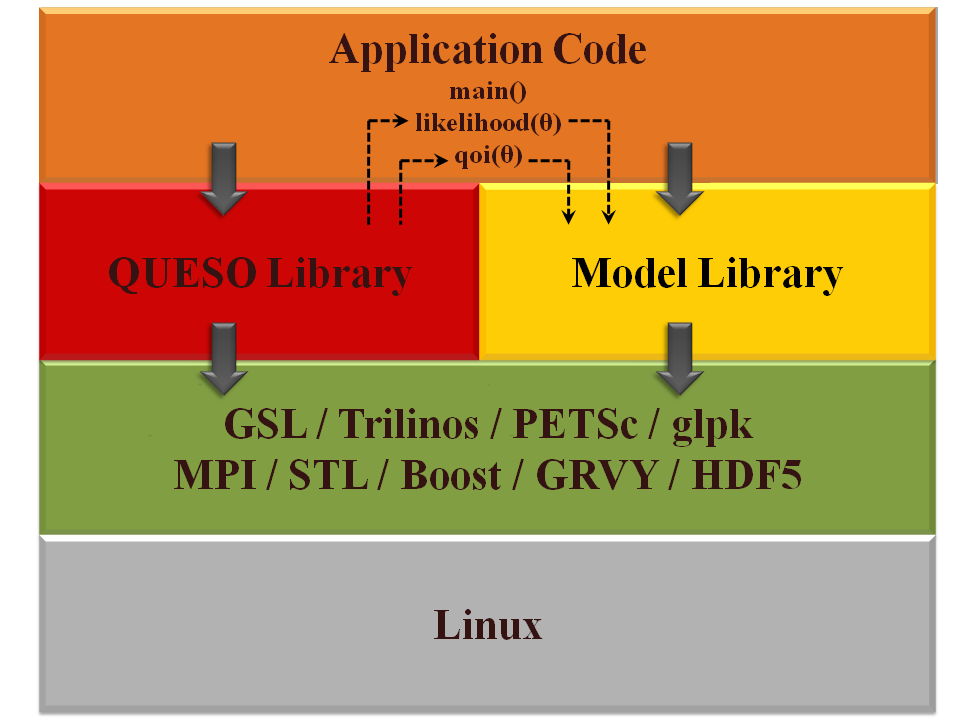
\includegraphics[scale=0.4,clip=true]{figs/quesoSwStack_09_2010.png}
}
\caption{
An application software stack.
QUESO requires the input
%supply
of a likelihood routine $\pi_{\text{like}}:\mathbb{R}^n\rightarrow\mathbb{R}_+$ for IPs and 
of a QoI routine $\mathbf{q}:\mathbb{R}^n\rightarrow\mathbb{R}^m$ for FPs.
These application level routines provide the bridge between
% among
the statistical algorithms in QUESO,
physics 
%model
knowledge in the model library, and relevant 
experimental (calibration
    and validation) data.
%model specific data in the disk space.
}
\label{fig-sw-stack}
\end{figure}

% \begin{figure}[h!]
% \centerline{
% 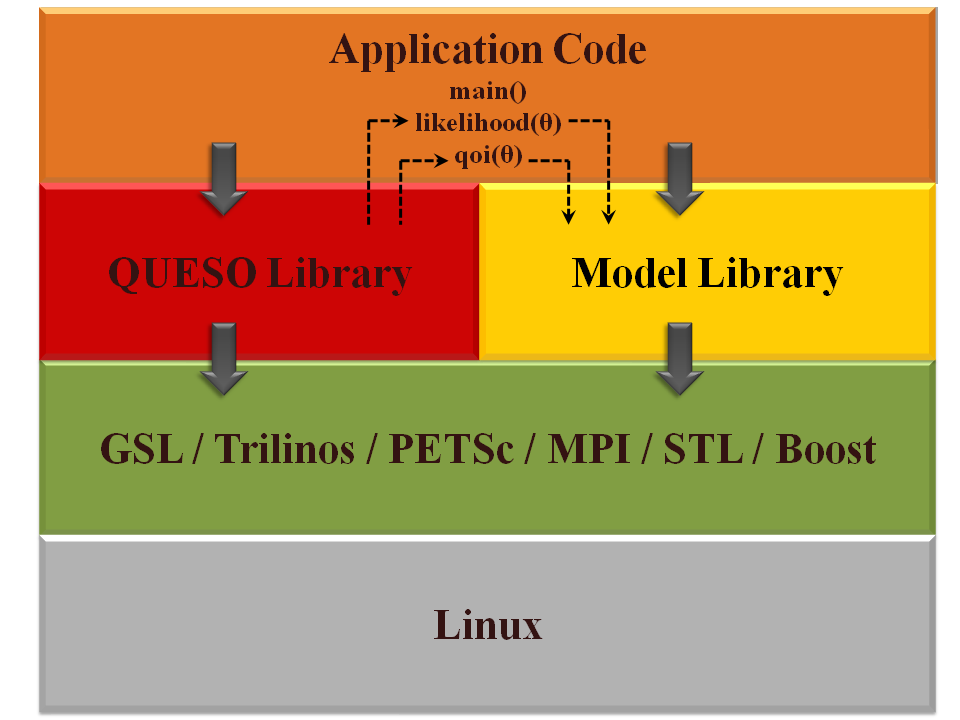
\includegraphics[scale=0.50,clip=true]{figs/queso_paper1_03}
% }
% \caption{
% Overview of the software stack of a typical application that uses QUESO.
% The symbol $\boldsymbol{\theta}$ represents a vector of $n\geqslant 1$ parameters.
% Algorithms in the QUESO library require the supply
% of a likelihood routine $\pi_{\text{like}}:\mathbb{R}^n\rightarrow\mathbb{R}_+$ for statistical inverse problems and 
% of a qoi routine $\mathbf{q}:\mathbb{R}^n\rightarrow\mathbb{R}^m$ for statistical forward problems. These routines
% exist at the application level and provide the necessary bridge between the statistical algorithms in QUESO,
% model knowledge in the model library and scenario and experimental data in the disk space.
% Concepts are further detailed in Chapter \ref{ch-introduction}.
% }
% \label{fig-sw-stack}
% \end{figure}
%
Even though QUESO deals directly with $\boldsymbol{\theta}$ and $\mathbf{q}$ only,
it is usually the case the one of the other three vectors ($\mathbf{u}$, $\mathbf{y}$ and $\mathbf{d}$) will have the biggest number of components and will therefore
dictate the size of the minimum parallel environment to be used in a problem.
%
So, for example, even though one processor might be sufficient for handling $\boldsymbol{\theta}$, $\mathbf{y}$, $\mathbf{d}$ and $\mathbf{q}$,
eight processors at least might be necessary to solve for $\mathbf{u}$.
QUESO currently only requires that the amounts $n$ and $m$ can be handled by the memory available to one processor,
which allows the analysis of problems with thousands of parameters and QoIs, a large amount even for state of the art UQ algorithms.

QUESO currently supports three modes of parallel execution:
an application user may simultaneously run:
\begin{description}
\item[(a)] multiple instances of a problem where the physical model requires a single processor, or
\item[(b)] multiple instances of a problem where the physical model requires multiple processors, or
\item[(c)] independent sets of types (a) and (b).
\end{description}

For example, suppose an user wants to use the Metropolis-Hastings (MH) algorithm to solve a statistical IP, and that 1,024 processors are available.
If the physical model is simple enough to be handled efficiently by a single processor, then the user can run 1,024 chains simultaneously, as in case (a).
If the model is more complex and requires, say, 16 processors, then the user can run 64 chains simultaneously, as in case (b), with 16 processors per chain.
QUESO treats this situation by using only 1 of the 16 processors to handle the chain.
When a likelihood evaluation is required, all 16 processors call the likelihood routine simultaneously.
Once the likelihood returns its value, QUESO puts  15 processors into idle state until the routine is called again or the chain completes.
Case (c) is useful, for instance, in the case of a computational procedure involving two models,
where a group of processors can be split into two groups, each handling one model.
Once the two-model analysis end, the combined model can use the full set of processors.\footnote{The parallel capabilities of QUESO have been exercised on the Ranger system of the TACC \cite{tacc} with up to 16k processors.}



\section{Algorithms for solving Statistical Inverse Problems}

The goal of inference is to characterize the posterior PDF, or to evaluate
point or interval estimates based on the posterior~\cite{HuMa01}.  Samples from
posterior can be obtained using Markov chain Monte Carlo (MCMC) which require
only pointwise evaluations of the unnormalized posterior.  The resulting
samples can then be used to either visually present the posterior or its
marginals, or to construct sample estimates of posterior expectations.
Examples of MCMC are: the Metropolis-Hastings (MH)
algorithm~\cite{Metr_1953,Hast_1970}, the Delayed Rejection (DR)
algorithm~\cite{GrMi01,Mira01}, and Adaptive Metropolis (AM)~\cite{HaSaTa01}
which are combined together in the Delayed Rejection Adaptive Metropolis, DRAM,
algorithm~\cite{HaLaMiSa06}. The DRAM is implemented in QUESO and available for
the solution of SIP. MCMC methods are well-established and
documented~\cite{CaSo07,GrMi01,HaLaMiSa06,HaSaTa01,Hast_1970,KaSo05,Laine08,Metr_1953,Mira01};
thus only brief description of the DRAM algorithm is presented in Section
\ref{sec:DRAM}. 


During model construction, errors arising from imperfect modeling and
uncertainties due to incomplete information about the system and its
environment always exist; thus, there has been a crescent interest in Bayesian
model class updating  and selection
\cite{ChingChen2007,ChOlPr10,CheungPrudencio2012}. 

Model updating refers to the methodology that determines the most plausible
model for a system, given a prior PDF. One stochastic method that handles model
updating successfully is the multilevel method. Throughout the years, sereveral
versions of the same method have been implemented as improvements of its
predecessors~\cite{BeckAu2002,ChingChen2007,CheungPrudencio2012}. QUESO hosts
the novel Adaptive Multilevel Stochastic Simulation Algorithm
(AMSSA)~\cite{CheungPrudencio2012}, which is described in Section
\ref{sec:ML:intro}. For details about the method, please refer to
\cite{CheungPrudencio2012}.

%\subsection{Markov chain Monte Carlo Algorithms}\label{sec:DRAM}


\subsection{DRAM Algorithm}\label{sec:DRAM}

DRAM is a combination of two ideas for improving the efficiency of
Metropolis-Hastings type Markov chain Monte Carlo (MCMC) algorithms, Delayed
Rejection and Adaptive Metropolis~\cite{DRAMtool}. 

Random walk Metropolis-Hasting algorithm with Gaussian proposal distribution is
useful in simulating from the posterior distribution in many Bayesian data
analysis situations.
% For example, in large class of nonlinear models we can write the model as
% $$
% y = f(x;\btheta) + \varepsilon,\quad     \varepsilon \sim \mathcal{N}(0,I \sigma^2),
% $$
% where $y$ are indepndent observations of the system, with the expected behaviour described by the model function $f(x;\btheta)$, depending on control variables $x$ and model parameters $\btheta$ distribution.
% 
In order for the chain to be efficient, the proposal covariance must somehow be
tuned to the shape and size of the target distribution. This is important in
highly nonlinear situations, when there are correlation between the components
of the posterior, or when the dimension of the parameter is high. The problem
of adapting the proposal distribution using the chain simulated so far is that
when the accepted values depend on the history of the chain, it is no longer
Markovian and standard convergence results do not apply. One solution is to use
adaptation only for the burn-in period and discard the part of the chain where
adaptation has been used. In that respect, the adaptation can be thought as
automatic burn-in. The idea of diminishing adaptation is that when adaptation
works well, its effect gets smaller and we might be able to prove the
ergodicity properties of the chain even when adaptation is used throughout the
whole simulation. This is the ideology behind AM adaptation. On the other hand,
the DR method allows the use of the the current rejected values without losing
the Markovian property and thus allows to adapt locally to the current location
of the target distribution.

In Adaptive Metropolis~\cite{HaSaTa01} the covariance matrix of the Gaussian
proposal distribution is adapted on the fly using the past chain. This
adaptation destroys the Markovian property of the chain, however, it can be
shown that the ergodicity properties of the generated sample remain. How well
this works on finite samples and on high dimension is not obvious and must be
verified by simulations.

Starting from initial covariance $C^{(0)}$, the target covariance is updated at
given intervals from the chain generated so far.
$$
%C_i = (cov(chain1:i) + I\delta)s,
C^{(i)} = s_d \, cov(\text{chain}_1:\text{chain}_i) + s_d \varepsilon I_d,
$$
the small number $\varepsilon$ prevents the sample covariance matrix from
becoming singular. For the scaling factor, the value $s_d = 2.4^2/d$ is
standard optimal choice for Gaussian targets, $d$ being the dimension of the
target~\cite{GelmanEtAl2004}. A standard updating formula for the sample
covariance matrix can be used, so that the whole chain does not need to reside
in the computer memory.

With the Delayed rejection method~\cite{Mira01}, it becomes possible to make
use of several tries after rejecting a value by using different proposals while
keep the reversibility of the chain. Delayed rejection method (DR) works in the
following way. Upon rejection a proposed candidate point, instead of advancing
time and retaining the same position, a second stage move is proposed. The
acceptance probability of the second stage candidate is computed so that
reversibility of the Markov chain relative to the distribution of interest is
preserved. The process of delaying rejection can be iterated for a fixed or
random number of stages, let's say $n_\text{stages}$. The higher stage
proposals are allowed to depend on the candidates so far proposed and rejected.
Thus DR allows partial local adaptation of the proposal within each time step
of the Markov chain still retaining the Markovian property and reversibility.

The first stage acceptance probability in DR is the standard MH acceptance and
it can be written as
\begin{equation*}
\alpha_1(\mathbf{a},\mathbf{x}^{(1)}) = \text{ min}
\left\{ 1,
\frac{\pi(\mathbf{x}^{(1)})}{\pi(\mathbf{a})} \cdot
\frac{q_1(\mathbf{x}^{(1)},\mathbf{a})}{q_1(\mathbf{a},\mathbf{x}^{(1)})}
\right\},
\end{equation*}

Here $\mathbf{a}$ is the current point, $\mathbf{x}^{(1)}$ is the proposed new
value drawn from the distribution $q_1(\mathbf{a}, \cdot)$, and $\pi$ is the
target distribution.  If $\mathbf{x}^{(1)}$ is rejected, a second candidate
$\mathbf{x}^{(2)}$ is drawn from $q_2(\mathbf{a}, \mathbf{x}^{(1)} , \cdot)$
using the acceptance probability
\begin{equation*}
\alpha_2( \mathbf{a}, \mathbf{x}^{(1)}, \mathbf{x}^{(2)}) =\min \left\{1,
\dfrac{\pi( \mathbf{x}^{(2)}) q_1( \mathbf{x}^{(2)}, \mathbf{x}^{(1)}) q_2( \mathbf{x}^{(2)}, \mathbf{x}^{(1)}, \mathbf{a})[1 - \alpha_1( \mathbf{x}^{(2)} , \mathbf{x}^{(1)} )]}{\pi( \mathbf{a}) q_1( \mathbf{a}, \mathbf{x}^{(1)}) q_2( \mathbf{a}, \mathbf{x}^{(1)}, \mathbf{x}^{(2)})[1 - \alpha_1 ( \mathbf{a}, \mathbf{x}^{(1)} )]}
\right\}
\end{equation*}
%
i.e., it depends not only on the current position of the chain but also on what
we have just proposed and rejected.

As the reversibility property is preserved, this method also leads to the same
stationary distribution $\pi$ as the standard MH algorithm. The procedure can
be iterated further for higher-stage proposals. 
%
The Gaussian proposal at each stage $i$ is defined as:
\begin{equation} % Gamma_i esta embutido na formula do q_i
\label{eq:qi}
q_i(\underbrace{\mathbf{a},\mathbf{x}^{(1)},\ldots,\mathbf{x}^{(i-1)}}_{i\text{ terms}},\mathbf{z})
=
e^{-\dfrac{1}{2}{\displaystyle \left\{[\mathbf{z}-\mathbf{a}]^T\cdot \left[\mathbf{C}\right]^{-1}\cdot[\mathbf{z}-\mathbf{a}]\right\}}} 
\end{equation}

% \begin{equation*} % Gamma_i esta embutido na formula do q_i
% q_i(\underbrace{\mathbf{a},\mathbf{x}^{(1)},\ldots,\mathbf{x}^{(i-1)}}_{i\text{ terms}},\mathbf{z})
% =
% e^{-\dfrac{1}{2}{\displaystyle \left\{[\mathbf{z}-\mathbf{a}]^T\cdot \left[\frac{1}{\gamma_i^2}\mathbf{C}\right]^{-1}\cdot[\mathbf{z}-\mathbf{a}]\right\}}} 
% \end{equation*}
where the covariance matrix $\mathbf{C}$ and the scalings for the higher-stage
proposal covariances
$1=\gamma_1\leqslant\gamma_2\leqslant\ldots\leqslant\gamma_{n_{\text{stages}}}$
are given.


If $q_i$ denotes the proposal at the $i$-th stage, the acceptance probability
at that stage is:
\begin{equation}\label{eq-alphas}
\alpha_i(\mathbf{a},\mathbf{x}^{(1)},\ldots,\mathbf{x}^{(i)}) = \text{ min}
\left\{1,
\frac {\pi(\mathbf{x}^{(i)})}{\pi(\mathbf{a})} \cdot q_{\text{fraction}} \cdot \alpha_{\text{fraction}}
\right\}.
\end{equation}
where the expressions $q_{\text{fraction}}$ and $\alpha_{\text{fraction}}$ are
given by
\begin{equation*}
q_{\text{fraction}}=
\frac{q_1(\mathbf{x}^{(i)},\mathbf{x}^{(i-1)})}{q_1(\mathbf{a},\mathbf{x}^{(1)})}
\frac{q_2(\mathbf{x}^{(i)},\mathbf{x}^{(i-1)},\mathbf{x}^{(i-2)})}{q_2(\mathbf{a},\mathbf{x}^{(1)},\mathbf{x}^{(2)})}
\ldots
\frac{q_i(\mathbf{x}^{(i)},\mathbf{x}^{(i-1)},\ldots,\mathbf{x}^{(1)},\mathbf{a})}{q_i(\mathbf{a},\mathbf{x}^{(1)},\ldots,\mathbf{x}^{(i-1)},\mathbf{x}^{(i)})}
\end{equation*}
and
\begin{equation*}
\alpha_{\text{fraction}}=
\frac{[1-\alpha_1(\mathbf{x}^{(i)},\mathbf{x}^{(i-1)})]}{[1-\alpha_1(\mathbf{a},\mathbf{x}^{(1)})]}
\frac{[1-\alpha_2(\mathbf{x}^{(i)},\mathbf{x}^{(i-1)},\mathbf{x}^{(i-2)})]}{[1-\alpha_2(\mathbf{a},\mathbf{x}^{(1)},\mathbf{x}^{(2)})]}
\ldots
\frac{[1-\alpha_{i-1}(\mathbf{x}^{(i)},\mathbf{x}^{(i-1)},\ldots,\mathbf{x}^{(1)})]}{[1-\alpha_{i-1}(\mathbf{a},\mathbf{x}^{(1)},\ldots,\mathbf{x}^{(i-1)})]}.
\end{equation*}


Since all acceptance probabilities are computed so that reversibility with
respect to $\pi$ is preserved separately at each stage, the process of delaying
rejection can be interrupted at any stage that is, we can, in advance, decide
to try at most, say, 3 times to move away from the current position, otherwise
we let the chain stay where it is. Alternatively, upon each rejection, we can
toss a p-coin (i.e., a coin with head probability equal to p), and if the
outcome is head we move to a higher stage proposal, otherwise we stay
put~\cite{HaLaMiSa06}.

The smaller overall rejection rate of DR guarantees smaller asymptotic variance
of the estimates based on the chain. The DR chain can be shown to be
asymptotically more efficient that MH chain in the sense of Peskun ordering
(Mira, 2001a). 

% Haario, et al. 2006 \cite{} combine AM and DR into a method called DRAM, in whzt they clain to me a straightforward possibility amonsgt the possible different implementations of the idea, which is decribed in this section.
% In order to be able to adapt the proposal at all you need some accepted points to start with. One ``master" proposal is tried first. After rejection, a try with modified version of the first proposal is done according to DR. A second proposal can be one with a smaller covariance, or with different orientation of the principal axes. The master proposal is adapted using the chain generated so far, and the second stage proposal follows the adaptation in obvious manner. %In the examples, and in the dramrun Matlab function, the second stage is just a scaled down version of the first stage proposal that itself is adapted according to AM. 
% 
% 
% The DRAM may be considered a straightforward way of combining AM adaptation with a $m$-stages DR algorithm, by doing:
% i) the proposal at the first stage of DR is adapted just as in AM: the covariance $C^{(1)}$  is computed from the points of the
% sampled chain, no matter at which stage these points have been accepted in the sample path;
% ii0 the covariance $C^{(i)}$  of the proposal for the $i$-th stage ($i=2,\ldots, m$) is always computed simply as a scaled version
% of the proposal of the first stage, $C^{(i)} = \gamma_i C^{(1)}$; where the scale factors $\gamma_i$ can be somewhat freely chosen.
% 
% ------------


Haario, et al. 2006 \cite{HaLaMiSa06} combine AM and DR into a method called
DRAM, in what they claim to be a straightforward possibility amongst the
possible different implementations of the idea, and which is described in this
section.

In order to be able to adapt the proposal, all you need some accepted points to
start with. 
%

One ``master" proposal is tried first -- i.e., the proposal at the first stage
of DR is adapted just as in AM: the covariance $C^{(1)}$  is computed from the
points of the sampled chain, no matter at which stage these points have been
accepted in the sample path.  After rejection, a try with modified version of
the first proposal is done according to DR. A second proposal can be one with a
smaller covariance, or with different orientation of the principal axes. The
most common choice is to always compute the covariance $C^{(i)}$  of the
proposal for the $i$-th stage ($i=2,\ldots, n_\text{stages}$) simply as a
scaled version of the proposal of the first stage, $$C^{(i)} = \gamma_i
C^{(1)}$$ where the scale factors $\gamma_i$ can be somewhat freely chosen.
Then, the master proposal is adapted using the chain generated so far, and the
second stage proposal follows the adaptation in obvious manner.

%In the examples, and in the dramrun Matlab function, the second stage is just a scaled down version of the first stage proposal that itself is adapted according to AM. 

The requirements for the DRAM algorithm are:
\begin{itemize}
 \item Number $n_{\text{pos}}\geqslant 2$ of positions in the chain;
 \item Initial guess $\mathbf{m}^{(0)}$;
 \item Number of stages for the DR method: $n_{\text{stages}}\geqslant 1$;
 \item For $1\leqslant i\leqslant n_{\text{stages}}$, functions $q_i:\underbrace{\mathbb{R}^N\times\ldots\times\mathbb{R}^N}_{(i+1)\text{ times}}\rightarrow\mathbb{R}_{+}$, such that $q_i(\mathbf{a},\mathbf{x}^{(1)},\ldots,\mathbf{x}^{(i-1)},\cdot)$ is a PDF for any $(\mathbf{a},\mathbf{x}^{(1)},\ldots,\mathbf{x}^{(i-1)})\in\underbrace{\mathbb{R}^N\times\ldots\times\mathbb{R}^N}_{i\text{ times}}$; i.e., choose $q_i$ as in Equation~\eqref{eq:qi};
 \item Recursively define $\alpha_i:\underbrace{\mathbb{R}^n\times\ldots\times\mathbb{R}^n}_{(i+1)\text{ times}}\rightarrow [0,1],\quad 1\leqslant i\leqslant n_{\text{stages}}$ according to Equation~\eqref{eq-alphas}.
\end{itemize}

% . Also, the Gaussian proposal at each stage $i$ is defined as:
% \begin{equation*}
% q_i(\underbrace{\mathbf{a},\mathbf{b},\ldots,\mathbf{y}}_{i\text{ terms}},\mathbf{z})
% =
% e^{-\frac{1}{2}{\displaystyle \left\{[\mathbf{z}-\mathbf{a}]^T\cdot \left[\frac{1}{\gamma_i^2}\mathbf{C}\right]^{-1}\cdot[\mathbf{z}-\mathbf{a}]\right\}}}
% \end{equation*}
% when the covariance matrix $\mathbf{C}$ and the ($n_{\text{stages}}$) numbers $1=\gamma_1\leqslant\gamma_2\leqslant\ldots\leqslant\gamma_{n_{\text{stages}}}$ are given.
% 

Recalling that a sample is defined as:
\begin{equation*} % Gamma_i may or may not be embedded in the covariance matrix
% \text{a sample } = \mathbf{a}+\frac{1}{\gamma_i}\mathbf{C}^{1/2}\mathcal{N}(0,I).
\text{a sample } = \mathbf{a}+\mathbf{C}^{1/2}\mathcal{N}(0,I).
\end{equation*}
a simple, but useful, implementation of DRAM is described in Algorithm \ref{alg:DRAM}.
 

\begin{algorithm}[!hp]
\SetLine
\SetLine
\KwIn{Number of positions in the chain $n_{\text{pos}}\geqslant 2$; initial guess $\mathbf{m}^{(0)}$; initial first stage proposal covariance $C^{(0)}$; $n_{\text{stages}}\geqslant 1$; and functions $q_i:\underbrace{\mathbb{R}^N\times\ldots\times\mathbb{R}^N}_{(i+1)\text{ times}}\rightarrow\mathbb{R}_{+}$}
% \KwOut{}

Select $s_d$                  \tcp*[r]{scaling factor} \nllabel{alg01_s}
Select $\varepsilon$        \tcp*[r]{covariance regularization factor} \nllabel{alg01_eps}
Select $n_0$                \tcp*[r]{initial non-adaptation period}

\For(\tcp*[f]{$n_{\text{stages}}$ is the number of tries allowed}){$i\leftarrow 1$ \KwTo $n_{\text{stages}}$}
  {Select $\gamma_i$ \tcp*[r]{scalings for the higher-stage proposal covariances}}   \nllabel{alg01_vf_ft}

\Repeat{ ($k+1 < n_{\text{pos}}$ ) }{ 
 Set $ACCEPT \leftarrow false$\;
 Set $i \leftarrow 1$\;

 \tcp{After an initial period of simulation, adapt the master proposal (target) covariance using the chain generated so far:}  
 \If{$k \geqslant n_0$}{
 $C^{(1)} = s_d Cov(\mathbf{m}^{(0)} ,\ldots, \mathbf{m}^{(k-1)}) + s_d \varepsilon I_d$\;
   }

 \tcp{$n_{\text{stages}}$-DR loop: }
 \Repeat{ (ACCEPT=false) and ($i \leqslant n_{\text{stages}}$)}{ %DR loop

Generate candidate $\mathbf{c}^{(i)}\in\mathbb{R}^N$ by sampling $q_i(\mathbf{m}^{(k)},\mathbf{c}^{(1)},\ldots,\mathbf{c}^{(i-1)},\cdot)$        \tcp*{$q_i$ is the proposal probability density}

\If {$\mathbf{c}^{(i)}\notin supp(\pi)$}{$i \leftarrow i+1 $}

\If {$\mathbf{c}^{(i)}\in supp(\pi)$}{ 
  Compute $\alpha_i(\mathbf{m}^{(k)},\mathbf{c}^{(1)},\ldots,\mathbf{c}^{(i-1)},\mathbf{c}^{(i)})$ \tcp*{acceptance probability} 
  
  Generate a sample $\tau \sim \mathcal{U}\left((0,1]\right ) $ %$0 < \tau\leqslant 1$ from an uniform rv defined over $(0,1]$\; 
  
  \lIf{ ($\alpha_i < \tau$)}{ $i\leftarrow i+1$}
  
  \lIf{ ($\alpha_i \geqslant\tau$)}{ACCEPT$\leftarrow$true}
  }

  $C^{(i)} = \gamma_i C^{(1)}$ \tcp*{Calculate the higher-stage proposal as scaled versions of~$C^{(1)}$, according to the chosen rule}
 
} %\Repeat{ (ACCEPT==false) and ($i \leqslant n_{\text{stages}}$)}{

\If{(\text{ACCEPT=true})}{ Set $\mathbf{m}^{(k+1)}\leftarrow \mathbf{c}^{(i)}$}

\If{(\text{ACCEPT=false})}{ Set $\mathbf{m}^{(k+1)} \leftarrow \mathbf{m}^{(k)}$}

Set $k \leftarrow k+1$\;

} % \Repeat{k+1 < n_{\text{pos}}}{

\caption{DRAM algorithm \cite{Laine08}.}\label{alg:DRAM}
\end{algorithm}



There are six variables in the QUESO input file used to set available options
for the DRAM algorithm, which are described in \ref{sec:MH}. Here, they are
presented presented bellow together with their respective definition in
Algorithm \ref{alg:DRAM}.
\begin{description}

 \item[\texttt{ip\_mh\_dr\_maxNumExtraStages}:] defines how many extra stages
   should be considered in the DR loop ($n_\text{stages}$);
 
 \item[\texttt{ip\_mh\_dr\_listOfScalesForExtraStages}:] defines the list $s$
   of scaling factors that will multiply the covariance matrix (values of
   $\gamma_i$ );
 
 
 \item[\texttt{ip\_mh\_am\_adaptInterval}:] defines whether or not there will
   be a period of adaptation;
   
   %the size of the interval in which each adapted proposal covariance matrix will be used;
 
 \item[\texttt{ip\_mh\_am\_initialNonAdaptInterval}:] defines the initial
   interval where the proposal covariance matrix will not be changed ($n_0$);
  
 \item[\texttt{ip\_mh\_am\_eta}:] is a factor used to scale the proposal
   covariance matrix, usually set to be $2.4^2/d$, where $d$ is the dimension
   of the problem~\cite{Laine08,HaLaMiSa06} ($s_d$);
 
 \item[\texttt{ip\_mh\_am\_epsilon}:] is the covariance regularization factor
   ($\varepsilon$).

\end{description}
%  
% ; they are presented and explained in details in Sections \ref{sec:MH} and \ref{sec:gravity-input-file}}. The three examples in Chapter \ref{chap:Queso-examples}, ``simpleStatisticalInverseProblem'', ``gravity'' and ``validation cycle'' use DRAM to solve their SIP. 


\subsection{Adaptive Multilevel Stochastic Simulation Algorithm}
\label{sec:ML:intro}


In this section we rewrite the Bayesian formula \eqref{eq-Bayes-solution} by
making explicit all the implicit model assumptions. Such explication demands
the use of probability logic and the concept of a stochastic system model class
(‘‘model class’’ for short); as these concepts enable the comparison of
competing model classes. 

Let $M_j$ be one model class; the choice of $\bv{\theta} $ specifies a
particular predictive model in $M_j$, and, for brevity, we do not explicitly
write $\bv{\theta}_j $ to indicate that the parameters of different model
classes may be different, but this should be understood.  Based on $M_j$, one
can use data $D$ to compute the updated relative plausibility of each
predictive model in the set defined by $M_j$.  This relative plausibility is
quantified by the \textit{posterior} PDF $\pi(\boldsymbol{\theta}|\D,M_j)$.


Bayes’ theorem allows the update of the probability of each predictive model
$M_j$ by combining measured data $D$ with the prior PDF into the posterior PDF:
\begin{equation}
\begin{split}
\pi_\post (\bv{\theta}|\D, M_j) &= \dfrac{f(\D|\bv{\theta}, M_j) \cdot \pi_\prior (\bv{\theta} | M_j)}{\pi(\D, M_j)} 
\\
&= \dfrac{f(\D|\bv{\theta}, M_j) \cdot \pi_\prior (\bv{\theta} | M_j)}{\int f(\D|\bv{\theta}, M_j) \cdot \pi_\prior (\bv{\theta} | M_j)\, d\bv{\theta}} 
\end{split}
\end{equation}
where the denominator expresses the probability of getting the data $\D$ based
on $M_j$ and is called the evidence for $M_j$ provided by $\D$;
$\pi_\prior (\bv{\theta} | M_j)$ is the prior PDF of the predictive model
$\bv{\theta}$ within $M_j$; and the likelihood function $f(\D|\bv{\theta}, M_j)$
expresses the probability of getting $\D$ given the predictive model
$\bv{\theta}$ within $M_j$ -- and this allows stochastic models inside a model
class $M_j$ to be compared. 




%\subsection{Intermediate distribution and evidence calculation}



When generating samples of posterior PDF $\pi_\post(\bv{\theta}|D,M_j) $ in
order to forward propagate uncertainty and compute QoI RV's, it is important to
take into account potential multiple modes in the posterior. One simple idea is
to sample increasingly difficult intermediate distributions, accumulating
``knowledge'' from one intermediate distribution to the next, until the target
posterior distribution is sampled.  In \cite{CheungPrudencio2012}, an advanced
stochastic simulation method, referred to as Adaptive Multi Level Algorithms,
is proposed which can generate posterior samples from
$\pi_\post (\bv{\theta}|\D, M_j)$ and compute the log of the evidence
$p(\D | \boldsymbol{\theta},M_j)$ at the same time by adaptively moving samples
from the prior to the posterior through an adaptively selected sequence of
intermediate distributions~\cite{ChOlPr10}.  

Specifically, the intermediate distributions are given by:
\begin{equation}
\label{eq:intermediate_dist}
\pi_\text{int}^{(\ell)} (\bv{\theta}|\D) = f(\bv{\theta}|\D, M_j)^{\tau_\ell} \cdot \pi_\prior (\bv{\theta} | M_j), \quad \ell=0,1,\ldots,L,
\end{equation}
for a given $L > 0$ and a given sequence $0 = \tau_0 < \tau_1 < \ldots < \tau_L = 1$
of exponents.


 

In order to compute the model evidence $\pi( \D |M_j)$ where:
\begin{equation}
 \label{eq:evidence}
 \pi( \D |M_j)=\int f(\bv{\theta}|\D, M_j) \cdot \pi_\prior (\bv{\theta}|M_j) \, d\bv{\theta}, 
\end{equation}
the use of intermediate distribution is also beneficial.
For that, recall that
\begin{equation}
\label{eq:cl}
\begin{split}
 \pi( \D |M_j) &= \int f(\bv{\theta})\pi (\bv{\theta}) \, d\bv{\theta} \\
  &= \int f \; \pi \, d\bv{\theta} \\
  &= \int f^{1-\tau_{L-1}} f^{\tau_{L-1}-\tau_{L-2}}\ldots f^{\tau_2-\tau_1} f^{\tau_1}\; \pi \, d\bv{\theta} \\
  &= c_1 \int f^{1-\tau_{L-1}} f^{\tau_{L-1}-\tau_{L-2}}\ldots f^{\tau_2-\tau_1} \dfrac{f^{\tau_1}\; \pi}{c_1} \, d\bv{\theta} \\
  &= c_2 c_1 \int f^{1-\tau_{L-1}} f^{\tau_{L-1}-\tau_{L-2}}\ldots  \dfrac{f^{\tau_2-\tau_1} f^{\tau_1}\; \pi}{c_2 c_1} \, d\bv{\theta} \\
  &= c_L c_{L-1} \cdots c_2 c_1.
\end{split}
\end{equation}
Assuming that the prior PDF is normalized (it integrates to one) and if
$\tau_{\ell}$ is small enough, then Monte Carlo method can be efficiently
applied to calculate $c_{\ell}$ in Equation \eqref{eq:cl}. Due to numerical
(in)stability, it is more appropriate to calculate the estimators:
\begin{equation}
 \label{eq:log-cl}
 \tilde{c_i} = \ln c_i, \quad i=1,\ldots, L.
\end{equation}

Combining Equations \eqref{eq:cl} and \eqref{eq:log-cl}, we have:
\begin{equation*}
 \ln[\pi( \D |M_j)] = \tilde{c}_{L}+\tilde{c}_{L-1}+\ldots+\tilde{c}_2+\tilde{c}_1.
\end{equation*}


Computing the log of the evidence instead of calculating the evidence directly
is attractive because the evidence is often too large or too small relative to
the computer precision.
%
The posterior probability can be calculated readily in terms of the log
evidence, allowing overflow and underflow errors to be avoided
automatically~\cite{ChOlPr10}.  
% In terms of the log evidence, the posterior
% probability is given by
% %
% \begin{equation} \label{ZEqnNumpost}
% P(M_j|D,M)=\frac{\exp[\ln \pi( \D |M_j)-E_{\max}]~P(M_j|M)}{\sum_{k=1}^{N_M}~\exp[\ln \pi( \D |M_k)-E_{\max}]~P(M_k|M)},
% \end{equation}
% %
% where $E_{\max}$ is the maximum of log evidences among the model classes in $M$:
% %
% \begin{equation} \label{maxln}
% E_{\max}=\max_{j\in[1,N_{M}]}\{\ln \pi( \D |M_j)\}.
% \end{equation}
% %


% \section{Auxiliary variables}

Now let's define some auxiliary variables for
$k=1,\ldots,n_\text{total}^{(\ell)}$:
    
    
\begin{itemize}
 \item $k$-th sample at the $\ell$-th level: 
    \begin{equation}\label{eq:samples}
    \bv{\theta}^{(\ell) [k]},   \quad \ell=0,1,\ldots, L \\ 
    \end{equation} 

 \item Plausibility weight:
    \begin{equation}
    \begin{split}\label{eq:w}
    w^{(\ell) [k]} &= \dfrac{f(\bv{\theta}^{(\ell) [k]}|\D, M_j)^{\tau_\ell} \cdot \pi_\prior (\bv{\theta}^{(\ell) [k]}, M_j)}{f(\bv{\theta}^{(\ell) [k]}|\D, M_j)^{\tau_\ell-1} \cdot \pi_\prior (\bv{\theta}^{(\ell) [k]}, M_j)}  
		=\dfrac{f^{(\tau_{\ell})}(\D | \bv{\theta}^{(\ell) [k]}, M_j) }{f^{(\tau_{\ell-1})}(\D | \bv{\theta}^{(\ell) [k]}, M_j)}, \\
		&= f^{(\tau_{\ell}-\tau_{\ell-1})}(\D | \bv{\theta}^{(\ell) [k]}, M_j), \quad \ell=0,1,\ldots, L \\ 
    \end{split}
    \end{equation}
    
\item Normalized plausibility weight:
    \begin{equation}\label{eq:w-tilde}
    \tilde{w}^{(\ell) [k]} = \dfrac{w^{(\ell) [k]}}{\sum_{s=1}^{n_\text{total}^{(\ell)}}  w^{(\ell) [s]} }, \quad \ell=0,1,\ldots,L 
    \end{equation}

\item Effective sample size:
    \begin{equation}\label{eq:neff}
    n_\text{eff}^{(\ell)} = \dfrac{1}{\sum_{s=1}^{n_\text{total}^{(\ell)}} \left( \tilde{w}^{(\ell) [s]}\right)^2}
    \end{equation}
    
\item Estimate for the sample covariance matrix for $\pi_\text{int}^{(\ell)}$:
    \begin{equation}\label{eq:est_cov}
     \Sigma = \sum_{m=1}^{n_\text{total}^{(\ell-1)}} \tilde{w}_{m} (\bv{\theta}^{(\ell-1) [m]} - \overline{\bv{\theta}}) (\bv{\theta}^{(\ell-1) [m]} - \overline{\bv{\theta}})^{t}, \quad \text{where} \quad
     \overline{\bv{\theta}} = \sum_{m=1}^{n_\text{total}^{(\ell-1)}}  \tilde{w}_{m} \bv{\theta}^{(\ell-1) [m]}
    \end{equation}

\end{itemize}


so we can define the discrete distribution:
\begin{equation}
 \label{eq:distribution}
 P^{(\ell)}(k) = \tilde{w}^{(\ell) [k]} , \quad k=1,2,\ldots, n_\text{total}^{(\ell)}.
\end{equation}


The ML algorithm consists of a series of resampling stages, with each stage
doing the following: given $n_\text{total}^{(\ell)}$ samples from
$\pi_\text{int}^{(\ell)} (\bv{\theta}|\D)$, denoted by
$\bv{\theta}^{(\ell)[k]}, k=1...n_\text{total}^{(\ell)}$ obtain samples from
$\pi_\text{int}^{(\ell+1)} (\bv{\theta}|\D)$, denoted by
$\bv{\theta}^{(\ell+1)[k]}, k=1...n_\text{total}^{(\ell+1)}$. 

This is accomplished by: given the samples
$\bv{\theta}^{(\ell)[k]}, k=1...n_\text{total}^{(\ell)}$, in Equation \eqref{eq:samples}, from
$\pi_\text{int}^{(\ell)} (\bv{\theta}|\D)$, we compute the plausibility weights
$w^{(\ell) [k]}$ given in Equation \eqref{eq:w} with respect to
$\pi_\text{int}^{(\ell+1)} (\bv{\theta}|\D)$. Then we re-sample the uncertain
parameters according to the normalized weights $\tilde{w}^{(\ell) [k]}$, given
in Equation \eqref{eq:w-tilde}, through the distribution in Equation
\eqref{eq:distribution}. This is possible due to the fact that for large
$n_\text{total}^{(\ell)}$ and $n_\text{total}^{(\ell+1)}$, then
$\bv{\theta}^{(\ell+1)[k]}, k=1...n_\text{total}^{(\ell+1)}$ will be
distributed as $\pi_\text{int}^{(\ell+1)}
(\bv{\theta}|\D)$~\cite{ChingChen2007}.

The choice of $\tau_\ell, \ell=1,\ldots,L-1$ is essential. It is desirable to
increase the $\tau$ values slowly so that the transition between adjacent PDFs
is smooth, but if the increase of the $\tau$ values is too slow, the required
number of intermediate stages ($L$ value) will be too
large~\cite{ChingChen2007}. More intermediate stages mean more computational
cost.  In the ML method proposed by \cite{CheungPrudencio2012} and implemented
in QUESO, $\tau_\ell$ is computed through a bissection method so that:
\begin{equation}\label{eq:tau}
\beta_\text{min}^{(\ell)}<\dfrac{n_\text{eff}^{(\ell)}}{n_\text{total}^{(\ell)}} <\beta_\text{max}^{(\ell)}
\end{equation}
%A common threshold is $\approx 0.9 \, n_\text{total}^{(\ell-1)}$ \cite{Cheung2008}.


\subsubsection{AMSSA Algorithm}

% Recall that for $\ell=0$, then $\pi_\text{int}^{(\ell)} (\bv{\theta}|\D)=\pi_\prior (\bv{\theta} | M_j)$ and for $\ell=L$ then $\pi_\text{int}^{(\ell)} (\bv{\theta}|\D)= \pi_\post(\bv{\theta}|\D, M_j)$, thus the series of intermediate PDFs start from the prior PDF and ends with the posterior PDF. 
Based on the above results, and recalling that the series of intermediate PDFs,
$\pi_\text{int}^{(\ell)} (\bv{\theta}|\D)$, start from the prior PDF and ends
with the posterior PDF,  Algorithm \ref{alg:ML} can be applied both to draw
samples from the posterior PDF, $\pi_\post (\bv{\theta}|\D, M_j)$, and to
estimate the evidence $\pi( \D ,M_j)$.

\begin{algorithm}[!htb]
%\AlFnt
\SetLine
\SetLine
\KwIn{for each $\ell=0,\ldots,L$: the total amount of samples to be generated at $\ell$-th level ($n_\text{total}^{(\ell)}>0$) and the thresholds ($0<\beta_\text{min}^{(\ell)}<\beta_\text{max}^{(\ell)}<1$) on the effective sample size of the $\ell$-th level}

%\KwOut{The n-th sample for $\bv{\theta}$ with the target PDF $\pi_\text{int}^{(\ell)}$. }

\KwOut{ $\bv{\theta}^{(m) [k]}, k=1,\ldots,n_\text{total}^{(m)}$; which are  asymptotically distributed as  $\pi_\post(\bv{\theta}|\D, M_j)$}

\KwOut{$\prod_{\ell} c_{\ell}$; which is asymptotically unbiased for $\pi( \D ,M_j)$ }

Set $\ell=0$\;                  

Set $\tau_\ell =0 $\;            

Sample prior distribution, $\pi_\prior (\bv{\theta} | M_j)$, $n_\text{total}^{(0)}$ times  \tcp*[r]{i.e, 
obtain $\bv{\theta}^{(0) [k]}, k=1,\ldots,n_\text{total}^{(0)}$}

\While{$\tau_\ell < 1$}{
 
 \tcc{At the beginning of the $\ell$-th level, we have the samples $\bv{\theta}^{(\ell-1)[k]}, k=1...n_\text{total}^{(\ell-1)}$ from  $\pi_\text{int}^{(\ell-1)} (\bv{\theta}|\D)$, Equation \eqref{eq:intermediate_dist}. }
 
 Set $\ell \leftarrow \ell + 1 $                  \tcp*[r]{begin next level}

 Compute plausibility weights $w^{(\ell) [k]}$ via Equation \eqref{eq:w}\;
 Compute normalized  weights $\tilde{w}^{(\ell) [k]}$ via Equation \eqref{eq:w-tilde}\;
 Compute $n_\text{eff}^{(\ell)}$ via Equation \eqref{eq:neff}\;

 Compute $\tau_\ell$ so that Equation \eqref{eq:tau} is satisfied\;
 \If{$\tau_\ell>1$}{
    $\tau_\ell \leftarrow 1$\;
    Recompute  $w^{(\ell) [k]}$ and  $\tilde{w}^{(\ell) [k]}$\;
 }
 
 Compute an estimate for the sample covariance matrix for $\pi_\text{int}^{(\ell)}$ via Equation \eqref{eq:est_cov}\;
 
%  Compute $c_{\ell} =\frac{1}{ n_\text{total}^{(\ell-1)}}  \left( \sum_{s=1}^{n_\text{total}^{(\ell-1)}} w_{s} \right)$ \tcp*[r]{recall that $\pi( \D |M_j) = \prod_{\ell} c_{\ell}$, Equation \eqref{eq:evidence}}
  
 Select, from previous level, the initial positions for the Markov chains\;  \nllabel{alg:ML:initialpos}

 Compute sizes of the chains         \tcp*[r]{the sum of the sizes $=n_\text{total}^{(\ell)}$} \nllabel{alg:ML:computechainsize}
 
 Redistribute chain initial positions among processors\; \nllabel{alg:ML:redist}
 
 \tcc{Then the $n_\text{total}^{(\ell)}$ samples $\bv{\theta}^{(\ell)[k]}$, from $\pi_\text{int}^{(\ell)}(\bv{\theta})$ are generated by doing the following for  $k=1,\ldots,n_\text{total}^{(\ell)}$:}

 Generate chains: draw a number $k'$ from a discrete distribution $P^{(\ell)}(k)$ in Equation \eqref{eq:distribution} via Metropolis-Hastings \tcp*[r]{i.e., obtain $\bv{\theta}^{(\ell) [k]}= P^{(l)[k]}$}
 
 Compute $c_{\ell} =\frac{1}{ n_\text{total}^{(\ell-1)}}  \left( \sum_{s=1}^{n_\text{total}^{(\ell-1)}} w_{s} \right)$ \tcp*[r]{recall that $\pi( \D |M_j) = \prod_{\ell} c_{\ell}$, Equation \eqref{eq:evidence}}
 
 }
\caption{Detailed description of the  Adaptive Multilevel Stochastic Simulation Algorithm proposed by \cite{CheungPrudencio2012}.}\label{alg:ML}
\end{algorithm}
% \todo{Line \ref{alg:ML:sampling} on Algorithm \ref{alg:ML} uses Metropolis-Hastings algorithm for sampling ; i.e., Generate $\bv{\theta}^*$ from a Gaussian PDF with mean $\bv{\theta}^{(\ell-1)[s']}$ and covariance $\Sigma$ from Equation \eqref{eq:est_cov} ... pagina 202 da tese}




%  
%  Using $\bv{\theta}^{(\ell-1)[s']}$ as the current sample, generate a sample $\bv{\theta}^{(\ell) [k]}$ for $\bv{\theta}$ by multi-group MCMC algorithms \nllabel{alg:ML:sampling} 
%  
%  Set $\bv{\theta}^{(\ell-1)[s']} =\bv{\theta}^{(\ell) [k]}$\;
%  \;
%  
%  \tcc{AQUI: ver Joseph's pagina 201/219}
%  Select, from previous level, the initial positions for the Markov chains \tcp*[r]{using samples from SSS as starting points}  \nllabel{alg:ML:initialpos}
 

% 
% \begin{algorithm}[!htb]
% \SetLine
% \SetLine
% \KwIn{for each $\ell=0,\ldots,L$: the total amount of samples to be generated at $\ell$-th level ($n_\text{total}^{(\ell)}>0$) and the thresholds ($0<\beta_\text{min}^{(\ell)}<\beta_\text{max}^{(\ell)}<1$) on the effective sample size of the $\ell$-th level}
% \KwOut{}
%  
% Set $\ell=0$\;                  
% Set $\tau_\ell =0 $\;            
% Sample prior distribution $n_\text{total}^{(0)}$ times  \tcp*[r]{i.e, obtain $\bv{\theta}^{(0) [k]}, k=1,\ldots,n_\text{total}^{(0)}$}
% 
% \While{$\tau_\ell < 1$}{
%  Set $\ell \leftarrow \ell + 1 $                         \tcp*[r]{begin next level}
%  Compute plausability weights $w^{(\ell) [k]}$ via Equation \ref{eq:w-tilde}
%  Compute $\tau_\ell$ so that $\beta_\text{min}^{(\ell)}<\dfrac{n_\text{eff}^{(\ell)}}{n_\text{total}^{(\ell)}} <\beta_\text{max}^{(\ell)}$\;
%  Select, from previous level, the initial positions for the Markov chains\;  \nllabel{alg:ML:initialpos}
%  Compute sizes of the chains                             \tcp*[r]{the sum of the sizes $=n_\text{total}^{(\ell)}$} 	\nllabel{alg:ML:computechainsize}
%  Redistribute chain initial positions among processors\; \nllabel{alg:ML:redist}
%  Generate chains\;
%  Compute $c_\ell$\;
%  }
% \caption{Multilevel algorithm \cite{}.}\label{alg:ML}
% \end{algorithm}

Steps \ref{alg:ML:initialpos} and \ref{alg:ML:computechainsize} in Algorithm
\ref{alg:ML} are accomplished by sampling the distribution in
Equation~\eqref{eq:distribution} a total of $n_\text{total}^{(\ell)} $ times.
The selected indices $k$ determine the samples $\bv{\theta}^{(\ell) [k]}$ to be
used as initial positions, and the number of times an index $k$ is selected
determines the size of the chain beginning at $\bv{\theta}^{(\ell) [k]}$.


At each level $\ell$, many computing nodes can be used to sample the parameter
space collectively. Beginning with $\ell = 0$, the computing nodes:
(a) sample $\pi_\text{int}^{(\ell)}(\bv{\theta}|\bv{D}, M_j)$; 
(b) select some of the generated samples (``knowledge'') to serve as initial positions of Markov chains for the next distribution $\pi_\text{int}^{(\ell+1)}(\bv{\theta}|\bv{D}, M_j)$; and 
(c) generate the Markov chains for $\pi_\text{int}^{(\ell+1)}(\bv{\theta}|\bv{D}, M_j)$. 

The process (a)--(b)--(c) continues until the final posterior distribution is
sampled.  As $\ell$ increases, the selection process tends to value samples
that are located in the regions of high probability content, which gradually
``appear''as  $\tau_\ell$ increases. So, as $\ell$ increases, if the ``good''
samples selected from the  $\ell$-th level to the ($\ell$+1)-th level are not
redistributed among computing nodes before the Markov chains for the (
$\ell$+1)-th level are generated, the ``lucky'' computing nodes (that is, the
ones that had, already at the initial levels, samples in the final posterior
regions of high probability content) will tend to accumulate increasingly more
samples in the next levels. This possible issue is avoided maintaining a
balanced computational load among all computing nodes, which is handled in the
ML by the step in Line \ref{alg:ML:redist}. 

Running the step in Line \ref{alg:ML:redist} of Algorithm \ref{alg:ML} is then
equivalent of solving the following problem: given the number of processors
$N_p$, the total number of runs $n_\text{total}$ and the number of runs $n_j$
(to be) handled by the $j$-th processor; distribute $N_t$ tasks among the $N_p$
processors so that each processor gets its total number $n_j$ of program runs,
$j = 1, \ldots, N_p$, the closest possible to the mean
$\bar{n}=n_\text{total}/N_p$. This parallel implementation of the algorithm is
proposed in \cite{CheungPrudencio2012}, and it has been implemented in QUESO by
the same authors/researchers.

% 
% There are several approaches in how to paralellize the multilevel algorithm~\cite{BeckAu2002,ChingChen2007,Angelikopoulos2012}. 
% The main problem in a straightforward parallel implementation, where each processor generates Markov chains independently for all $\tau_j$, is load imbalance.  Markov chains assigned to processors exploring high probability regions of the parameter space must generate a larger number of samples than those processors exploring low probability regions, leading to load imbalance as $\alpha_i \rightarrow 1$.  Thus, an important feature of the parallel implementation is the load
% balancing at each point in the $\tau_j$ sequence.  The parallel implementation of the algorithm is proposed in \cite{CheungPrudencio2012}, and it is implemented in QUESO by the same authors/researchers. The redistribution of the initial chain positions among the processors is represented by step \ref{alg:ML:redist} of on Algorithm \ref{alg:ML}. 







\section{Algorithms for solving the Statistical Forward Problem}

The Monte Carlo method is commonly used for analyzing uncertainty propagation,
where the goal is to determine how random variation, lack of knowledge, or
error affects the sensitivity, performance, or reliability of the system that
is being modeled \cite{RoCa04}.

Monte Carlo works by using random numbers to sample, according to a PDF, the
`solution space' of the problem to be solved.  Then, it iteratively evaluates a
deterministic model using such sets of random numbers as inputs.

%aken from http://www.physics.buffalo.edu/phy411-506/topic2/topic2-lec2.pdf
Suppose we wish to generate random numbers distributed according to a positive
definite function in one dimension $P(x)$.  The function need not be normalized
for the algorithm to work, and the same algorithm works just as easily in a
many dimensional space. The random number sequence $x_i$, $i=0,1,2,\ldots$ is
generated by a random walk as follows:

\begin{enumerate}
\item Choose a starting point $x_0$
\item Choose a fixed maximum step size $\delta$.
\item Given a $x_i$,  generate the next random number as follows: 
  \begin{enumerate}
  \item Choose $x_\text{trial}$  uniformly and randomly in the interval $[x_i-\delta, x_i+\delta]$.
  \item Compute the ratio $w=\dfrac{P(x_\text{trial})}{P(x_i)}$.
 
   Note that $P$ need not be normalized to compute this ratio.
  
  \item If $w >1$ the trial step is in the  right direction, i.e., towards a region of higher probability. 
  
  Accept the step $x_{i+1} =x_\text{trial}$.
  
  \item  If $w <1$ the trial step is in the wrong direction, i.e., towards a region of lower probability.  We should not unconditionally reject this step! So accept the step conditionally if the decrease in probability is smaller than a random amount:
     \begin{enumerate}
     \item Generate a random number $r$ in the interval $[0,1]$.
     \item If $r < w$ accept the trial step $x_{i+1} = x_\text{trial}$.
     \item If $w \leq r $ reject the step $x_{i+1}=x_i$. Note that we don't discard this step! The two steps have the same value.
     \end{enumerate}
  \end{enumerate}
\end{enumerate}

There are essentially two important choices to be made.  First, the initial
point $x_0$ must be chosen carefully. A good choice is close to the maximum of
the desired probability distribution. If this maximum is not known (as is
usually the case in multi-dimensional problems), then the random walker must be
allowed to thermalize i.e., to find a good starting configuration: the
algorithm is run for some large number of steps which are then discarded.
Second, the step size must be carefully chosen. If it is too small, then most
of the trial steps will be accepted, which will tend to give a uniform
distribution that converges very slowly to $P(x)$. If it is too large the
random walker will step right over and may not ` `see" important peaks in the
probability distribution. If the walker is at a peak, too many steps will be
rejected. A rough criterion for choosing the step size is for the
$$ \text{Acceptance ratio} = \dfrac{\text{Number of steps accepted}}{\text{Total number of trial steps}}$$
to be around 0.5.

An implementation of Monte Carlo algorithm is described in Algorithm
\ref{alg:MC}.


\begin{algorithm}[!htb]
%\AlFnt
\SetLine
\SetLine
\KwIn{Starting point $x_0$, step size $\delta$, number of trials $M$, number of steps per trial $N$, unnormalized density or probability function  $P(x)$ for the target distribution.}

\KwOut{Random number sequence $x_i$, $i=0,1,2,\ldots$}

\For{$i=0...M$}{
  \For{$j=0...N$}{

  Set $ x_\text{trial} \leftarrow  x_i + (2 \, \text{RAND([0,1])} - 1)  \delta$\;
  Set $ w = P(x_\text{trial}) / P(x) $\;
  Set $accepts \leftarrow 0$\;

  \eIf(\tcp*[h]{uphill}){$w \geq 1$}
  {
    $x_{i+1} \leftarrow x_\text{trial} $  \tcp*[r]{accept the step}
    accepts $\leftarrow$ accepts+1\;
  }
  (\tcp*[h]{downhill}) %else
  { 
    Set $r \leftarrow$ RAND([0,1])\;
      \If(\tcp*[h]{but not too far}){$ r < w$}{
	$ x_{i+1} \leftarrow x_\text{trial} $  \tcp*[r]{accept the step}
	accepts $\leftarrow$ accepts+1\;
      }
  }
}
}

\caption{Detailed description of the Monte Carlo Algorithm proposed by \cite{Metr_1953}.}\label{alg:MC}
\end{algorithm}


Monte Carlo is implemented in QUESO and it is the chosen algorithm to compute a
sample of the output RV (the QoI) of the SFP for each given sample of the input
RV. 
